\documentclass[12pt]{article}
\setlength\parindent{0pt}
\usepackage{fullpage}
\usepackage{amsmath}
\usepackage{graphicx}
\setlength{\parskip}{4mm}
\def\LL{\left\langle}   % left angle bracket
\def\RR{\right\rangle}  % right angle bracket
\def\LP{\left(}         % left parenthesis
\def\RP{\right)}        % right parenthesis
\def\LB{\left\{}        % left curly bracket
\def\RB{\right\}}       % right curly bracket
\def\PAR#1#2{ {{\partial #1}\over{\partial #2}} }
\def\PARTWO#1#2{ {{\partial^2 #1}\over{\partial #2}^2} }
\def\PARTWOMIX#1#2#3{ {{\partial^2 #1}\over{\partial #2 \partial #3}} }
\newcommand{\BE}{\begin{displaymath}}
\newcommand{\EE}{\end{displaymath}}
\newcommand{\BNE}{\begin{equation}}
\newcommand{\ENE}{\end{equation}}
\newcommand{\BEA}{\begin{eqnarray}}
\newcommand{\EEA}{\nonumber\end{eqnarray}}
\newcommand{\EL}{\nonumber\\}
\newcommand{\la}[1]{\label{#1}}
\newcommand{\ie}{{\em i.e.\ }}
\newcommand{\eg}{{\em e.\,g.\ }}
\newcommand{\cf}{cf.\ }
\newcommand{\etc}{etc.\ }
\newcommand{\Tr}{{\rm tr}}
\newcommand{\etal}{{\it et al.}}
\newcommand{\OL}[1]{\overline{#1}\ } % overline
\newcommand{\OLL}[1]{\overline{\overline{#1}}\ } % double overline
\newcommand{\OON}{\frac{1}{N}} % "one over N"
\newcommand{\OOX}[1]{\frac{1}{#1}} % "one over X"



\begin{document}
\Large
\centerline{\sc{Recitation Questions}}
\normalsize
\centerline{\sc{Week of 22 February}}

\begin{enumerate}



\begin{enumerate}
  \item{A person uses a rope to spin a bucket of mass 800g in a vertical circle at a constant speed; the radius of the circle is 125 cm. The bucket goes around the circle once every second.}
    \begin{enumerate}
      \item{What is the tension in the rope at the top of the circle?}
      \item{What is the tension in the rope at the bottom of the circle?}
    \end{enumerate}

  \item{A person swings a cup of water in a vertical circle at a constant speed using his arm, If the length of the person's arm is $L$, how fast must the person swing the cup so that the water does not fall out? Give your answer in terms of $L$ and $g$.}

  \item{Knight problem 8.36, reproduced here:\\}
    \centerline{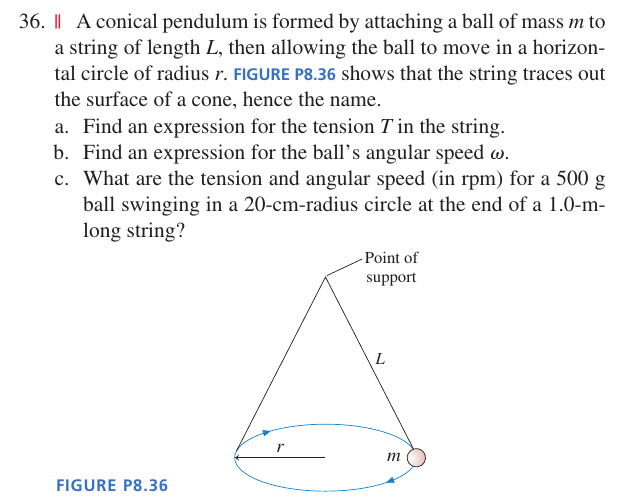
\includegraphics[width=0.6\textwidth]{conical-pendulum.png}}

  \item{A highway curve has a radius of curvature of 500 meters; that is, it is a segment of a circle whose radius is 500 m. It is banked so that traffic moving at 30 m/s can travel
  around the curve without needing any help from friction.}

\begin{enumerate}
  
  \item{What banking angle of the curve achieves this?}

\end{enumerate}

\item{We say that $g=9.81\,\rm m/\rm s^2$, but this varies slightly from place to place on Earth. Mt. Everest is about 9 km above sea level; how much does $g$ decrease from gaining
  9 km of altitude?}

\item{Compute the mass of the Sun. The Earth's orbit is very nearly circular, and the earth is 150 million km from the Sun. Here are some steps you might take as a guide:}
  \begin{enumerate}
    \item{What is the angular velocity of the Earth in its orbit?}
    \item{What is the tangential velocity of the Earth?}
    \item{What is the radial acceleration of the Earth?}
    \item{What is the mass of the Sun?}
  \end{enumerate}


\item{As you saw in the previous problem dealing with a person in an elevator, 
    your ``apparent weight'' is the normal force the ground exerts on your feet. If you stand on the Equator, how much does your apparent weight differ from your true weight due to the 
    rotation of the Earth? (Hint: What is your acceleration here?}
\end{enumerate}
\end{document}
